\documentclass[11pt]{report}

\usepackage[utf8]{inputenc}
\usepackage[T1]{fontenc}
\usepackage[francais]{babel}

\usepackage{hyperref}
\usepackage{tikz}
\usepackage{amsmath,amssymb}
\usepackage{graphicx}
\usepackage{array}
\usepackage{color}
\usepackage{subfigure}
\usepackage{caption}
\usepackage{booktabs}
\usepackage{threeparttable}
\usepackage{amsmath}
\usepackage{array}
\usepackage{tabularx}
\usepackage{lmodern} % police Latin Modern
\usepackage{hyperref}
\usepackage{fancyhdr}
\usepackage{listingsutf8}
\usepackage{verbatim}
\usepackage[autolanguage]{numprint}
\usepackage{rotating}
\usepackage[top=3cm, bottom=3cm, left=3cm, right=3cm]{geometry}
\pagestyle{fancy}
\addto\captionsfrench{\def\tablename{Tableau}}
\lhead{Stegen Thomas s154315 \quad  Adrien Minne s154340 \quad  Delaunoy Arnaud s153059}
\hypersetup{                    % parametrage des hyperliens
    colorlinks=true,                % colorise les liens
    breaklinks=true,                % permet les retours à la ligne pour les liens trop longs
    urlcolor= black,                 % couleur des hyperliens
    linkcolor= black,                % couleur des liens internes aux documents (index, figures, tableaux, equations,...)
    citecolor= green                % couleur des liens vers les references bibliographiques
    }
\definecolor{mygreen}{RGB}{28,172,0} % color values Red, Green, Blue
\definecolor{mylilas}{RGB}{170,55,241}
\title{Processus stochastiques : cryptanalyse}
\author{Stegen Thomas s154315 \\ Adrien Minne s154340 \\ Delaunoy Arnaud s153059}
\date{}
\renewcommand\thesection{\arabic{section}}
\renewcommand\thesubsection{\arabic{section}.\arabic{subsection}}
\renewcommand\thesubsubsection{Question \arabic{subsubsection}}
\begin{document}
\setcounter{secnumdepth}{3}
\lstset{
language=matlab,
keywordstyle=\color{blue},
morekeywords=[2]{1}, keywordstyle=[2]{\color{black}},
identifierstyle=\color{black},
stringstyle=\color{mylilas},
commentstyle=\color{mygreen},
numberstyle={\tiny \color{black}},
emph=[1]{for,end,break},emphstyle=[1]\color{blue},
}
 \lstset{%
            inputencoding=utf8,
                breaklines=true,
                extendedchars=true,
                literate=%
                {é}{{\'e}}{1}%
                {è}{{\`e}}{1}%
                {à}{{\`a}}{1}%
                {ç}{{\c{c}}}{1}%
                {œ}{{\oe}}{1}%
                {ù}{{\`u}}{1}%
                {É}{{\'E}}{1}%
                {È}{{\`E}}{1}%
                {À}{{\`A}}{1}%
                {Ç}{{\c{C}}}{1}%
                {Œ}{{\OE}}{1}%
                {Ê}{{\^E}}{1}%
                {ê}{{\^e}}{1}%
                {î}{{\^i}}{1}%
                {ô}{{\^o}}{1}%
                {û}{{\^u}}{1}%
                {ë}{{\¨{e}}}1
                {û}{{\^{u}}}1
                {â}{{\^{a}}}1
                {Â}{{\^{A}}}1
                {Î}{{\^{I}}}1
        }

\begin{titlepage}
\maketitle
\end{titlepage}
\section{ Première partie : chaines de Markov pour la modélisation du langage et MCMC}
\subsection{Chaine de Markov pour la modélisation du langage}
\subsubsection{}
L'élément (i,j) de la matrice de transition correspond à la probabilité de passer de l'état i à l'état j. Il correspond donc à la probabilité que la lettre i soit suivie de la lettre j dans la séquence. Dès lors, soit $\theta$ l'élément (i,j) de la matrice de transition, $\theta$ est le paramètre d'une loi de Bernouilli avec comme possibilités:
\begin{itemize}
\item l'élément i est suivi de j (avec une probabilité $\theta$)
\item l'élément i n'est pas suivi de j (avec une probabilité $1-\theta$)
\end{itemize}
\paragraph{}
La méthode du maximum de vraisemblance consiste à maximiser $P(\bf{D}_n|\theta)$ avec $\bf{D}_n$ l'échantillon de donnée, ici seq1 et n le nombre de données. Pour une variable de Bernouilli, on a: Soit,\\ 
$$
\mbox{} x_i = \left\{
    \begin{array}{ll}
        1 & \mbox{si i est suivi de j} \\
        0 & \mbox{si i n'est pas suivi de j}
    \end{array}
\right.
$$
et m le nombre d’occurrences de la lettre i.
\begin{align*}
P(\bf{D}_n|\theta) &= \prod_{i = 1}^{m} (x_i \theta +(1-x_i)(1-\theta)) \\
                   &= \theta^{n_1} (1-\theta)^{n_0}
\end{align*}
Avec $n_0$ le nombre de fois où $x_i = 0$ et $n_1$ le nombre de fois où $x_i = 1$. Déterminons maintenant le $\theta$ maximisant cette fonction:
\begin{align*}
\frac{\partial P(\bf{D}_n|\theta)}{\partial \theta} 
&= n_1 \theta^{n_1-1} (1-\theta)^{n_0} - n_1\theta^{n_1} (1-\theta)^{n_0-1} \\
&= \theta^{n_1-1} (1-\theta)^{n_0-1} (n_1 (1-\theta) - n_0 \theta) \\
&= \theta^{n_1-1} (1-\theta)^{n_0-1} (n_1 - \theta (n_1 + n_0))
\end{align*}
La valeur de $\theta$ maximisant la fonction $P(\bf{D}_n|\theta)$ est donc:
$$ \theta_{i,j} = \frac{n_1}{n_0+n_1} = \frac{\mbox{nombre d'occurrences de i suivies de j}}{\mbox{nombre d'occurrences de i}} $$
\subsubsection{}
Cette question est résolue par la fonction \texttt{estimate\_prob}. La t-ième puissance de Q est simplement calculée avec l'opérateur exposant de matlab.\\
Pour le calcul de $P(X_t = x)$, on calcule $\pi(t) = \pi(0)*Q^t$ avec $\pi(0) = (0.25\ 0.25\ 0.25\ 0.25)$ dans le cas ou la première lettre est choisie au hasard et $\pi(0) = (0\ 0\ 1\ 0)$ quand la première lettre est c. $P(X_t = x)$ est l'élément de $\pi(t)$ correspondant à x (le premier pour a, le deuxième pour b, ...).\\
L'évolution de la probabilité est reprise sur les graphiques \ref{prob_a}, \ref{prob_b}, \ref{prob_c} et \ref{prob_d}. On constate qu'en t = 0, elle est uniquement dépendante de $\pi(0)$, ce qui est normal au vu de la définition de $\pi(0)$. Quand t augmente, la probabilité est de moins en moins dépendante de $\pi(0)$ et dépend donc de plus en plus de la matrice de transition. C'est en accord avec la théorie car quand le temps augmente, la distribution tend vers la distribution stationnaire si $Q^t$ converge vers une valeur limite pour $t \rightarrow +\infty$. C'est le cas ici car 
$$Q^{1000} = Q^{1001} =
\begin{bmatrix}
0.3518 & 0.0754 & 0.2161 & 0.3568\\
0.3518 & 0.0754 & 0.2161 & 0.3568\\
0.3518 & 0.0754 & 0.2161 & 0.3568\\
0.3518 & 0.0754 & 0.2161 & 0.3568
\end{bmatrix}
$$ 
\begin{figure}[!h]
\begin{center}
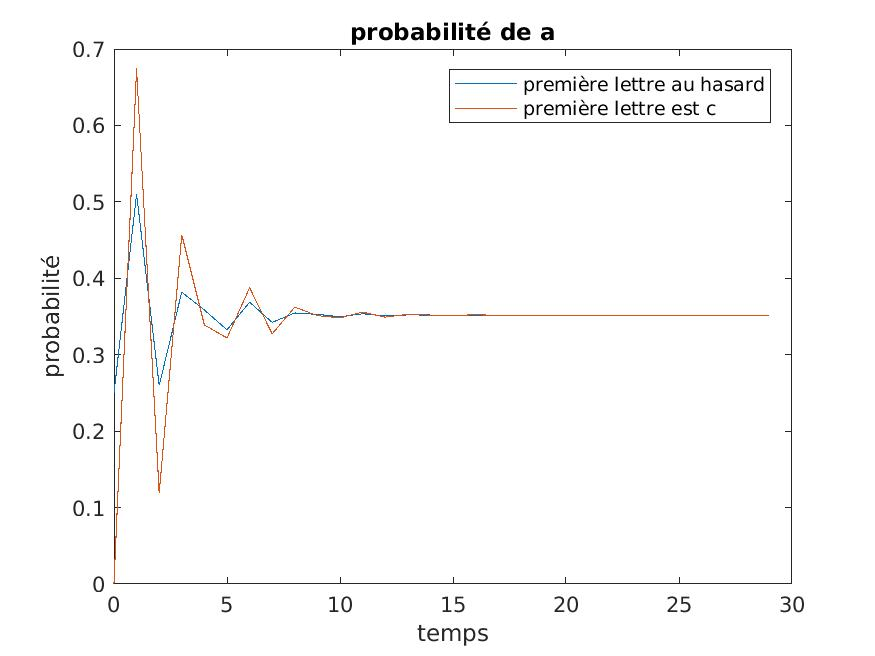
\includegraphics[height = 9cm]{prob_a.jpg}
\caption{\label{prob_a}}
\end{center}
\end{figure}
\begin{figure}[!h]
\begin{center}
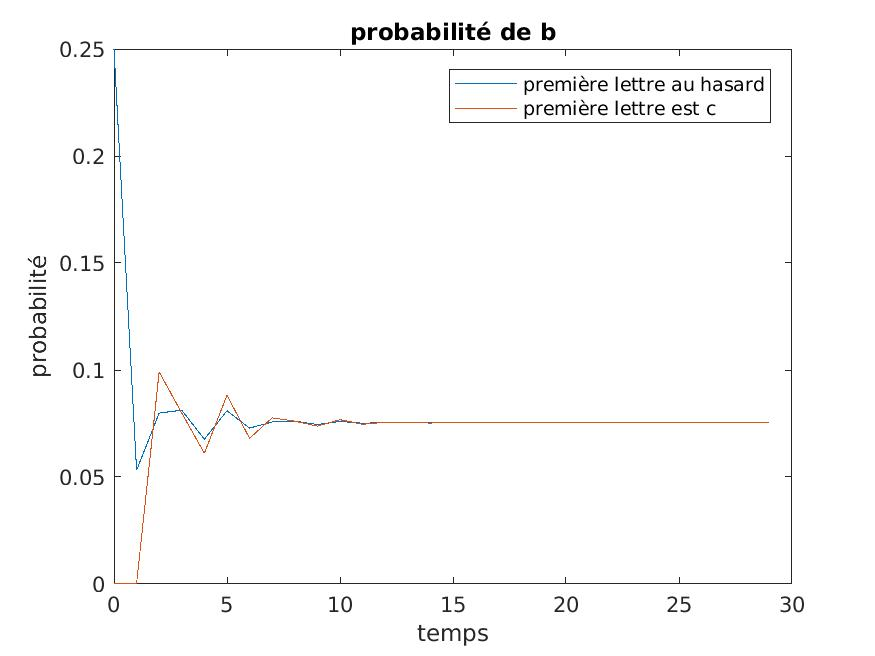
\includegraphics[height = 9cm]{prob_b.jpg}
\caption{\label{prob_b}}
\end{center}
\end{figure}
\begin{figure}[!h]
\begin{center}
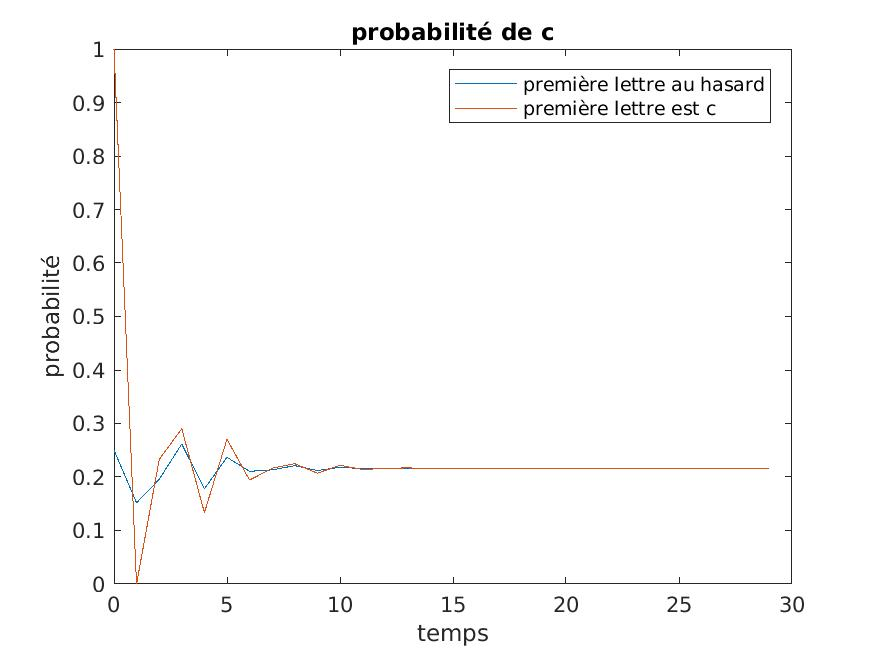
\includegraphics[height = 9cm]{prob_c.jpg}
\caption{\label{prob_c}}
\end{center}
\end{figure}
\begin{figure}[!h]
\begin{center}
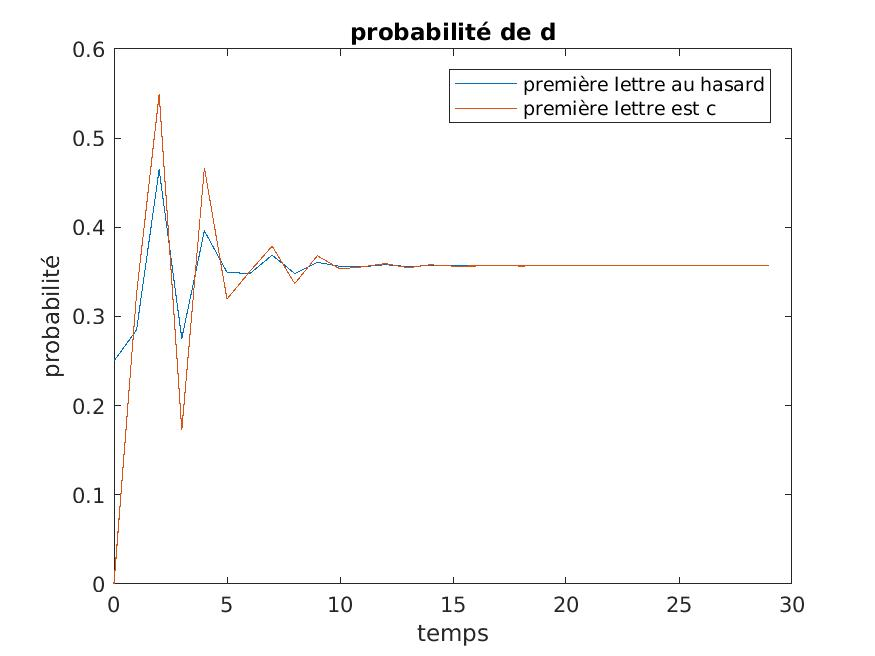
\includegraphics[height = 9cm]{prob_d.jpg}
\caption{\label{prob_d}}
\end{center}
\end{figure}
\subsubsection{}
\subsubsection{}
\subsubsection{}
\subsection{Algorithme MCMC}
\subsubsection{}
Pour prouver que $\pi_0$ est une distribution stationnaire de la chaine de Markov, il suffit de prouver que $\pi_0=\pi_0 *Q$. 
On sait que les équations de balances détaillées $\pi_0(i)Q_{i,j} = \pi_0(j)Q_{j,i}$ sont satisfaites.
Passant en notation indicielle, on doit donc montrer que :
\begin{align*}
\pi_0(i) &= \sum^{N}_{k=0} \pi_0(k)*Q_{k,i} \\
& = \sum^{N}_{k=0} \pi_0(i)*Q_{i,k} \\
& = \pi_0(i) \sum^{N}_{k=0} \pi_0(i) Q_{i,k} \\
& = \pi_0(i)
\end{align*}
Cette distribution stationnaire est unique si la matrice de transition Q est irréductible.
\subsubsection{}
Cette démonstration a été faite avec l'aide du pdf nommé MetropolisExplanation mis dans l'archive trouvé sur internet.\\
Étudions d'abord la probabilité de transition.\\
La probabilité d'obtenir un élément $x_j$ sachant que l'élément précédent de la chaîne de Markov est $x_i$ est pour $i \neq j$ la probabilité que cet élément soit généré selon la loi q et accepté.
$$P(x_j | x_i) = \alpha(x_j, x_i) q(x_j| x_i)$$
avec
\begin{align*}
\alpha(x_j, x_i) 
&= min \left\{1, \frac{f(x_j)}{f(x_i)} \frac{q(x_i|x_j)}{q(x_j|x_i)}\right\}\\
&= min \left\{1, \frac{cP_X(x_j)}{cP_X(x_i)} \frac{q(x_i|x_j)}{q(x_j|x_i)}\right\}
\end{align*}
La probabilité d'obtenir à nouveau l'élément $x_i$ sachant que l'élément précédent de la chaîne de Markov est également $x_i$ est la somme de la probabilité que l'élément $x_i$ soit généré selon la loi q et accepté et de la probabilité que tout autre élément soit généré et refusé.
$$P(x_i | x_i) = \alpha(x_i, x_i) q(x_i|x_i) + \sum_k (1-\alpha(x_k, x_i)) q(x_k |x_i)$$

Dans le cas où l'élément généré est différent du précédent, on a:
\begin{align*}
P(x_j | x_i) \pi_0(x_i)
&= \alpha(x_j, x_i) q(x_j| x_i) \pi_0(x_i) \\
&= min \left\{1, \frac{cP_X(x_j)}{cP_X(x_i)} \frac{q(x_i|x_j)}{q(x_j|x_i)}\right\} q(x_j| x_i) \pi_0(x_i) \\
&= \frac{\pi_0(x_i)}{cP_X(x_i)} min \left\{cP_X(x_i) q(x_j|x_i), cP_X(x_j) q(x_i|x_j)\right\} \\
&\text{en posant } x_i \leftarrow x_j \text{ et } x_j \leftarrow x_i \\
&= \frac{\pi_0(x_j)}{cP_X(x_j)} min \left\{cP_X(x_j) q(x_i|x_j), cP_X(x_i) q(x_j|x_i)\right\} \\
&= min \left\{1, \frac{cP_X(x_i)}{cP_X(x_j)} \frac{q(x_j|x_i)}{q(x_i|x_j)}\right\} q(x_i| x_j) \pi_0(x_j)\\
&= \alpha(x_i, x_j) q(x_i| x_j) \pi_0(x_j) \\
&= P(x_i | x_j) \pi_0(x_j)
\end{align*} 

Dans le cas où l'élément généré est le même que le précédent, $x_i$ étant égal à $x_j$ il est évident que 
$$P(x_i | x_j) \pi_0(x_j) = P(x_j | x_i) \pi_0(x_i)$$
car 
$$P(x_i | x_i) \pi_0(x_i) = P(x_i | x_i) \pi_0(x_i)$$
\section{Deuxième partie : décryptage d’une séquence codée}
\subsubsection{}
Pour déterminer la cardinalité de l'ensemble $\Theta$, il suffit de calculer le nombre possibles de permutations des caractères disponibles. On considère la langue anglaise avec 40 caractèresle nombre de permutations possibles, on considère qu'on a 40 permutatations possibles pour la première lettre, 39 pour la deuxième, ... On a donc : 
$$|\Theta| = 40 * 39 *38 * ... * 1!$$. 
\subsubsection{}
\paragraph{}
Dans le modèle $\pi_0, Q$, on peut trouver la vraisemblance de la séquence $T'$ en mutlipliant les probabilité d'avoir la lettre $n$ de $T'$ en partant de la lettre $n-1$ de $T'$. Nos probabilités sont calculées comme suit : 

\begin{itemize}
\item $P(lettre 1 = T'(1))$ est simplement sa probabilité d'avoir cette lettre dans $\pi_{0}$.
\item $P(lettre 2 = T'(2))$ : est la probabilité d'avoir cette lettre dans $\pi_{0}*Q$.
\item $P(lettre 3 = T'(3))$ : est la probabilité d'avoir cette lettre dans $\pi_{0}*Q^{2}$.
\item etc
\end{itemize}

La vraisemblance de la chaine $T'$ est donc, notant N la taille de la chaine $T'$ et $| \pi|_{T'(k)}$ la probabilité d'avoir la $k^{ième}$ lettre de $T'$ selon la distribution $\pi$ :
$$P(T') = \prod_{k=0}^{N} |\pi_{0}*Q^{k}|_{T'(k)}$$

\paragraph{}
Pour trouver la vraisemblance de $D$, il faut d'abord calculer la matrice $Q_{\theta}$ exprimant notre matrice Q dans le cas  de la permutation $\theta$. Ensuite, la vraisemblance de $D$ se trouve de la même facon que celle de $T'$, à savoir : 
$$P(D) = \prod_{k=0}^{N} |\pi_{0}*Q_{\theta}^{k}|_{D(k)}$$

\subsubsection{}

Si il n'a que 10 codes candidats possible qui ont la même probabilité, il est assez simple de retrouver le texte de base. Il suffit en effet de calculer la vraisemblance de notre texte avec chaque code $\theta$ suivant l'algorithme décrit au point 2.2, et puis simplmenet sélectionner le $\theta$ menan	t au texte ayant la plus grande vraisemblance.
\subsubsection{}
\subsubsection{}
\subsubsection{}
\end{document}